%%%%%%%%%%%%%%%%%%%%%%%%%%%%%%%%%%%%%%%%%
% Beamer Presentation
% LaTeX Template
% Version 1.0 (10/11/12)
%
% This template has been downloaded from:
% http://www.LaTeXTemplates.com
%
% License:
% CC BY-NC-SA 3.0 (http://creativecommons.org/licenses/by-nc-sa/3.0/)
%
%%%%%%%%%%%%%%%%%%%%%%%%%%%%%%%%%%%%%%%%%

%----------------------------------------------------------------------------------------
%	PACKAGES AND THEMES
%----------------------------------------------------------------------------------------

\documentclass{beamer}

\mode<presentation> {

% The Beamer class comes with a number of default slide themes
% which change the colors and layouts of slides. Below this is a list
% of all the themes, uncomment each in turn to see what they look like.

%\usetheme{default}
%\usetheme{AnnArbor}
%\usetheme{Antibes}
%\usetheme{Bergen}
%\usetheme{Berkeley}
%\usetheme{Berlin}
%\usetheme{Boadilla}
%\usetheme{CambridgeUS}
%\usetheme{Copenhagen}
%\usetheme{Darmstadt}
%\usetheme{Dresden}
%\usetheme{Frankfurt}
%\usetheme{Goettingen}
%\usetheme{Hannover}
%\usetheme{Ilmenau}
%\usetheme{JuanLesPins}
%\usetheme{Luebeck}
\usetheme{Madrid}
%\usetheme{Malmoe}
%\usetheme{Marburg}
%\usetheme{Montpellier}
%\usetheme{PaloAlto}
%\usetheme{Pittsburgh}
%\usetheme{Rochester}
%\usetheme{Singapore}
%\usetheme{Szeged}
%\usetheme{Warsaw}

% As well as themes, the Beamer class has a number of color themes
% for any slide theme. Uncomment each of these in turn to see how it
% changes the colors of your current slide theme.

%\usecolortheme{albatross}
%\usecolortheme{beaver}
%\usecolortheme{beetle}
%\usecolortheme{crane}
%\usecolortheme{dolphin}
%\usecolortheme{dove}
%\usecolortheme{fly}
%\usecolortheme{lily}
%\usecolortheme{orchid}
%\usecolortheme{rose}
%\usecolortheme{seagull}
%\usecolortheme{seahorse}
%\usecolortheme{whale}
%\usecolortheme{wolverine}
\usepackage{mathrsfs}



%\setbeamertemplate{footline} % To remove the footer line in all slides uncomment this line
%\setbeamertemplate{footline}[page number] % To replace the footer line in all slides with a simple slide count uncomment this line

%\setbeamertemplate{navigation symbols}{} % To remove the navigation symbols from the bottom of all slides uncomment this line
}
\usepackage{CJKutf8}
\usepackage{graphicx} % Allows including images
\usepackage{booktabs} % Allows the use of \toprule, \midrule and \bottomrule in tables

% UTF-8 encoding
% CJKfonts package
% latex+dvips, latex+dvipdfm(x) or pdflatex


\AtBeginSection[]
{
	\begin{frame}<beamer>
		\frametitle{Outline for section \thesection}
		{\scriptsize \tableofcontents[ currentsection ]}
	\end{frame}
}
%\tableofcontents[ 
%currentsubsection, 
%hideothersubsections, 
%sectionstyle=show/hide, 
%subsectionstyle=show/shaded, 
%]
\begin{document}
\begin{CJK*}{UTF8}{bsmi}

%\documentclass{article}
%----------------------------------------------------------------------------------------
%	TITLE PAGE
%----------------------------------------------------------------------------------------

\title[A Fuzzy Association Rule-Based Classification
Model for High-Dimensional Problems With
Genetic Rule Selection and Lateral Tuning]{A Fuzzy Association Rule-Based Classification
Model for High-Dimensional Problems With
Genetic Rule Selection and Lateral Tuning} % The short title appears at the bottom of every slide, the full title is only on the title page

\author{鍾岳峰} % Your name
\institute[Yue-Fong,Chung] % Your institution as it will appear on the bottom of every slide, may be shorthand to save space
{
元智大學 \\ % Your institution for the title page
\medskip
\textit{pchomekimojuf@gmail.com} % Your email address
}
\date{\today} % Date, can be changed to a custom date



\begin{frame}
\titlepage % Print the title page as the first slide
\end{frame}



\begin{frame}{Outline}
%\begin{frame}[allowframebreaks]{Outline}
\frametitle{Overview} % Table of contents slide, comment this block out to remove it

\tableofcontents[hideallsubsections] % Throughout your presentation, if you choose to use \section{} and \subsection{} commands, these will automatically be printed on this slide as an overview of your presentation
%\framebreak
%\tableofcontents{2}
\end{frame}

%----------------------------------------------------------------------------------------
%	PRESENTATION SLIDES
%----------------------------------------------------------------------------------------

%------------------------------------------------
\section{INTRODUCTION} % Sections can be created in order to organize your presentation into discrete blocks, all sections and subsections are automatically printed in the table of contents as an overview of the talk
%第一章介紹
%------------------------------------------------

% A subsection can be created just before a set of slides with a common theme to further break down your presentation into chunks

%提示%%%%%%%%%%%%%%%%%%%%%%%%%%%%%%%%%%%%%
%****要做重點劃紅線可以用
%{\color{red}fuzzy measures} 
%****草寫
% \Large $\mathscr{B}$
%換行
%\\
%提示%%%%%%%%%%%%%%%%%%%%%%%%%%%%%%%%%%%%%

%------------------------------------------------

\begin{frame}
	\frametitle{\insertsection : \insertsubsection}
	
	\begin{itemize}
		\item FUZZY rule-based classification systems (FRBCSs) are useful and well-known tools in the machine learning framework, since they can provide an interpretable model for the end user . 
		
		\item Association discovery is one of the most common data mining techniques that are used to extract interesting knowledge from large datasets.
		
		\item Much effort has been made to use its advantages for classification under the name of associative classification.
		
	\end{itemize}
	
\end{frame}

%------------------------------------------------
%------------------------------------------------

\begin{frame}
	\frametitle{\insertsection : \insertsubsection}
	\begin{itemize}
		\item Both association discovery and classification rules mining are essential in practical data mining applications , and their integration could result in greater savings and convenience for the user.
		\item A typical associative classification system is constructed in two stages:
	\end{itemize}
	\begin{block}{ }
		
		~\\
		1) discovering the association rules inherent in a database; \\
		2) selecting a small set of relevant association rules to construct a classifier.\\
		~\\
	\end{block}
	
\end{frame}

%------------------------------------------------

%------------------------------------------------

\begin{frame}
	\frametitle{\insertsection : \insertsubsection}
	\begin{itemize}
		\item In this paper, we present a fuzzy association rule-based classification method for high-dimensional problems (FARC-HD) to obtain an accurate and compact fuzzy rule-based classifier with a low computational cost.
		\item This method is based on the following three stages:
	\end{itemize}
	\begin{block}{ }
		
		~\\
		1) Fuzzy association rule extraction for classification.\\
		2) Candidate rule prescreening.\\
		3) Genetic rule selection and lateral tuning\\
		~\\
	\end{block}
	\begin{itemize}
	\item In order to assess the performance of the proposed approach, we have used 26 real-world datasets with a number of variables ranging from 4 to 90 and a number of patterns ranging from 150 to 19,020.
	\end{itemize}
\end{frame}

%------------------------------------------------


\section{PRELIMINARIES}
\subsection{A.Fuzzy Rule-Based Classification Systems}

%------------------------------------------------

\begin{frame}
\frametitle{\insertsection : \insertsubsection}
	\begin{itemize}
		\item Any classification problem consists of N training patterns, i.e., $\mathit{x}_{p}$ = ($\mathit{x}_{p1}$,...,$\mathit{x}_{pm}$), $\mathit{p}$ = 1,2,...,N, from S classes, where $\mathit{x}_{pi}$ is the $\mathit{i}$th attribute value ($\mathit{i}$ = 1,2,...,$\mathit{m}$) of the pth training pattern.
		\item  In this paper, we use fuzzy rules of the following form for our classifier:
	\end{itemize}
	\begin{block}{ }
~\\
\centering\textbf{Rule ~$\mathit{R}_{j}$:IF~$\mathit{A}_{j1}$ and ··· and $\mathit{x}_{m}$ is $\mathit{A}_{jm}$}\\
\centering\textbf{THEN Class = $\mathit{C}_{j}$ with $\mathit{RW}_{j}$}\\
~\\
\end{block}

\end{frame}

%------------------------------------------------
%------------------------------------------------

\begin{frame}
	\frametitle{\insertsection : \insertsubsection}

	\begin{block}{ (1)}
		~\\
	\centering\textbf{${RW}_{\mathit{j}} = {CF}_{\mathit{j}}=\dfrac{\sum_{x_{p} \in ClassC_{j}}^{} {\mu A_{j}(x_{p})}}{\sum_{p=1}^{N} {\mu A_{j}(x_{p})}}$}\\
		~\\
	\end{block}
		\begin{block}{ (2)}
			~\\
			\centering\textbf{${V}_{Class_\mathit{h}}(x_{p}) = \sum_{R_{j} \in RB ; R_{j}=\mathit{h}}^{} {\mu A_{j} (x_{p}) \bullet CF_{\mathit{j}}}$}\\
		~\\
		~~~~~~~~~~~~~	\textbf{$\mathit{h}=1,2,...,S,$~~~~$R_{\mathit{j}} \in RB.$}\\
			
			~\\
		\end{block}
	
\end{frame}

%------------------------------------------------


\subsection{B.Fuzzy Association Rules}

%------------------------------------------------

\begin{frame}
	\frametitle{\insertsection : \insertsubsection}
\begin{center}
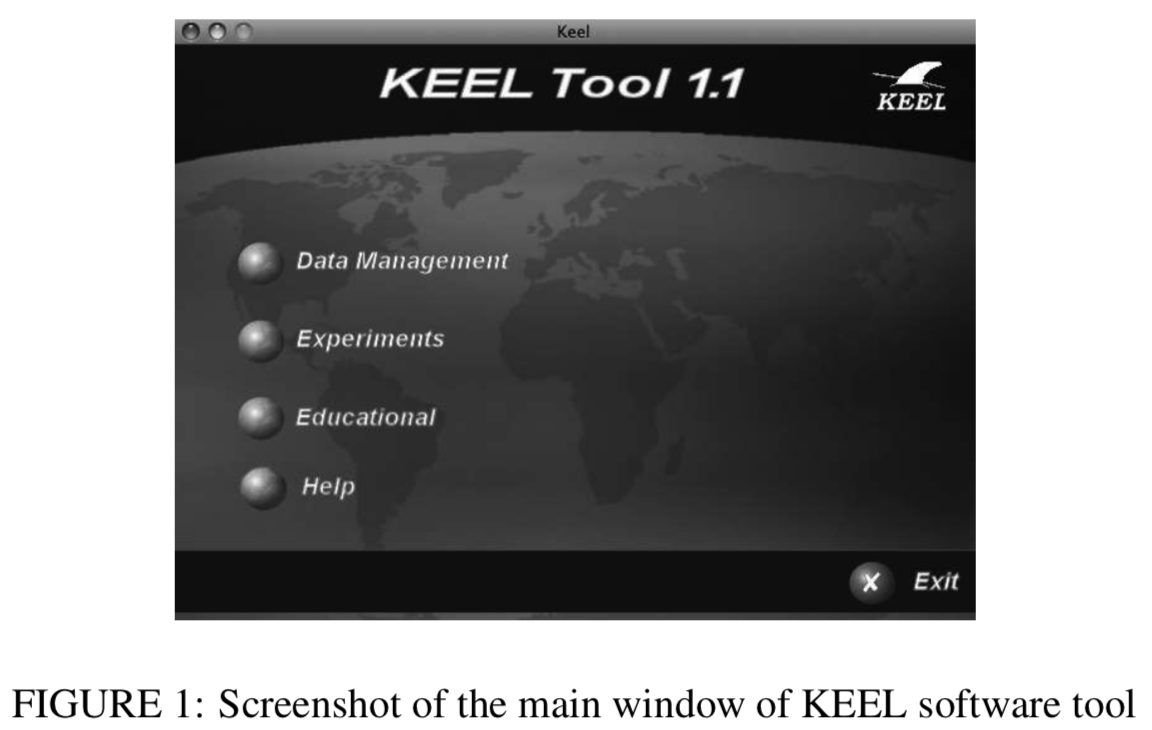
\includegraphics[width=1\linewidth]{./1.png}
\end{center}
\end{frame}

%------------------------------------------------
%------------------------------------------------

\begin{frame}
	\frametitle{\insertsection : \insertsubsection}
	
	\begin{block}{ (3)}
		~\\
		\centering\textbf{$Support(A\longrightarrow B)=\dfrac{\sum_{x_{p}\in T}^{ }{\mu {AB}(x_{p})}}{|N|}$}\\
		~\\
	\end{block}
	\begin{block}{ (4)}
		~\\
		\centering\textbf{$Confidence(A\longrightarrow B)=\dfrac{\sum_{x_{p}\in T}^{ }{\mu {AB}(x_{p})}}{\sum_{x_{p}\in T}^{ }{\mu {A}(x_{p})}}$}\\
		~\\

		~\\
	\end{block}
	
\end{frame}

%------------------------------------------------

\subsection{C.Fuzzy Association Rules for Classification}

%------------------------------------------------

\begin{frame}
	\frametitle{\insertsection : \insertsubsection}
	
	\begin{block}{ (5)}
		~\\
		\centering\textbf{$Support(A\longrightarrow C_{j})=\dfrac{\sum_{x_{p}\in ClassC_{j}}^{ }{\mu A(x_{p})}}{|N|}$}\\
		~\\
	\end{block}
	\begin{block}{ (6)}
		~\\
		\centering\textbf{$Confidence(A\longrightarrow C_{j})=\dfrac{\sum_{x_{p}\in ClassC_{j}}^{ }{\mu A(x_{p})}}{\sum_{x_{p}\in T}^{ }{\mu A(x_{p})}}$}\\
		~\\
		
		~\\
	\end{block}
	
\end{frame}

%------------------------------------------------

\section{FUZZY ASSOCIATION RULE-BASED CLASSIFIER FOR HIGH-DIMENSIONAL  PROBLEMS}
\subsection{Stage 1. Fuzzy Association Rule Extraction for Classification}

%------------------------------------------------

\begin{frame}
	\frametitle{\insertsection : \insertsubsection}
\begin{center}
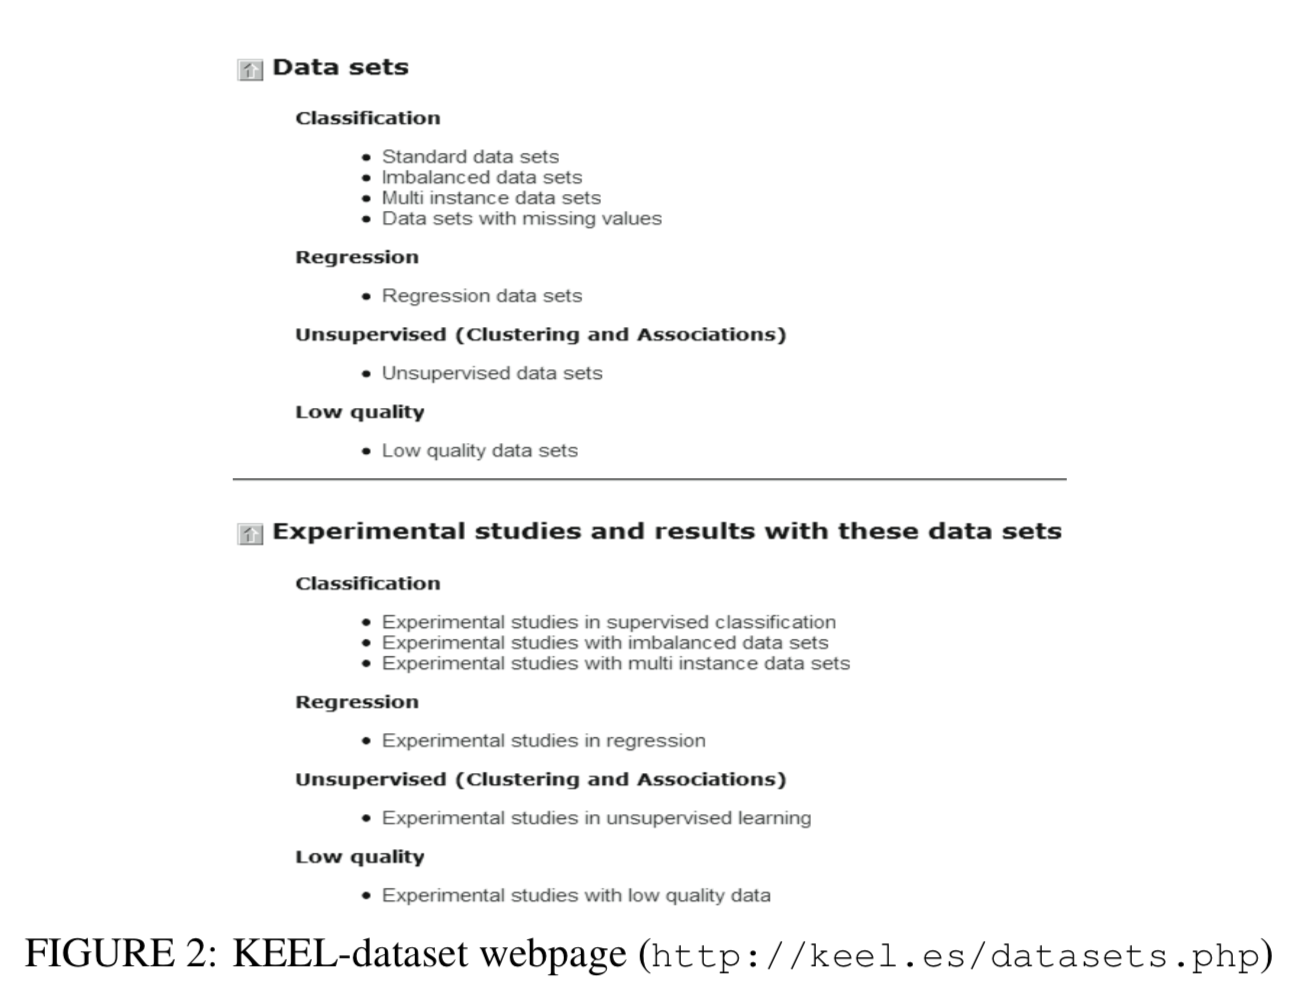
\includegraphics[width=1\linewidth]{./2.png}
\end{center}
\end{frame}

%------------------------------------------------
%------------------------------------------------

\begin{frame}
	\frametitle{\insertsection : \insertsubsection}
	
	\begin{block}{ (7)}
		~\\
		\centering\textbf{$Support(A)=\dfrac{\sum_{x_{p}\in T}^{ }{\mu A(x_{p})}}{|N|}$}\\
		~\\
	\end{block}
	\begin{block}{ (8)}
		~\\
		\centering\textbf{$MinimumSupport_{C_{j}}=minSup\ast \mathit{f}_{C_{j}}$}\\
		~\\
	\end{block}
	
\end{frame}

%------------------------------------------------

\subsection{Stage 2. Candidate Rule Prescreening}

%------------------------------------------------

\begin{frame}
	\frametitle{\insertsection : \insertsubsection}
	
	\begin{block}{ (9)}
		~\\
		\centering\textbf{$wWRAcc'  (A\longrightarrow C_{j})=\dfrac{n'(A)}{N'}\bullet(\dfrac{n'(A\bullet C_{j})}{n'(A)}-\dfrac{n(C_{j})}{N})$}\\
		~\\
	\end{block}
		\begin{itemize}
			\item N′ is the sum of the weights of all patterns.
			\item n′(A) is the sum of the weights of all covered patterns .
			\item n′(A · $C_{j}$ ) is the sum of the weights of all correctly covered patterns.
			\item n($C_{j}$ ) is the number of patterns of class $C_{j}$.  
			\item N is the number of all patterns. 
			
		\end{itemize}
	
\end{frame}

%------------------------------------------------
%------------------------------------------------

\begin{frame}
	\frametitle{\insertsection : \insertsubsection}
\begin{center}
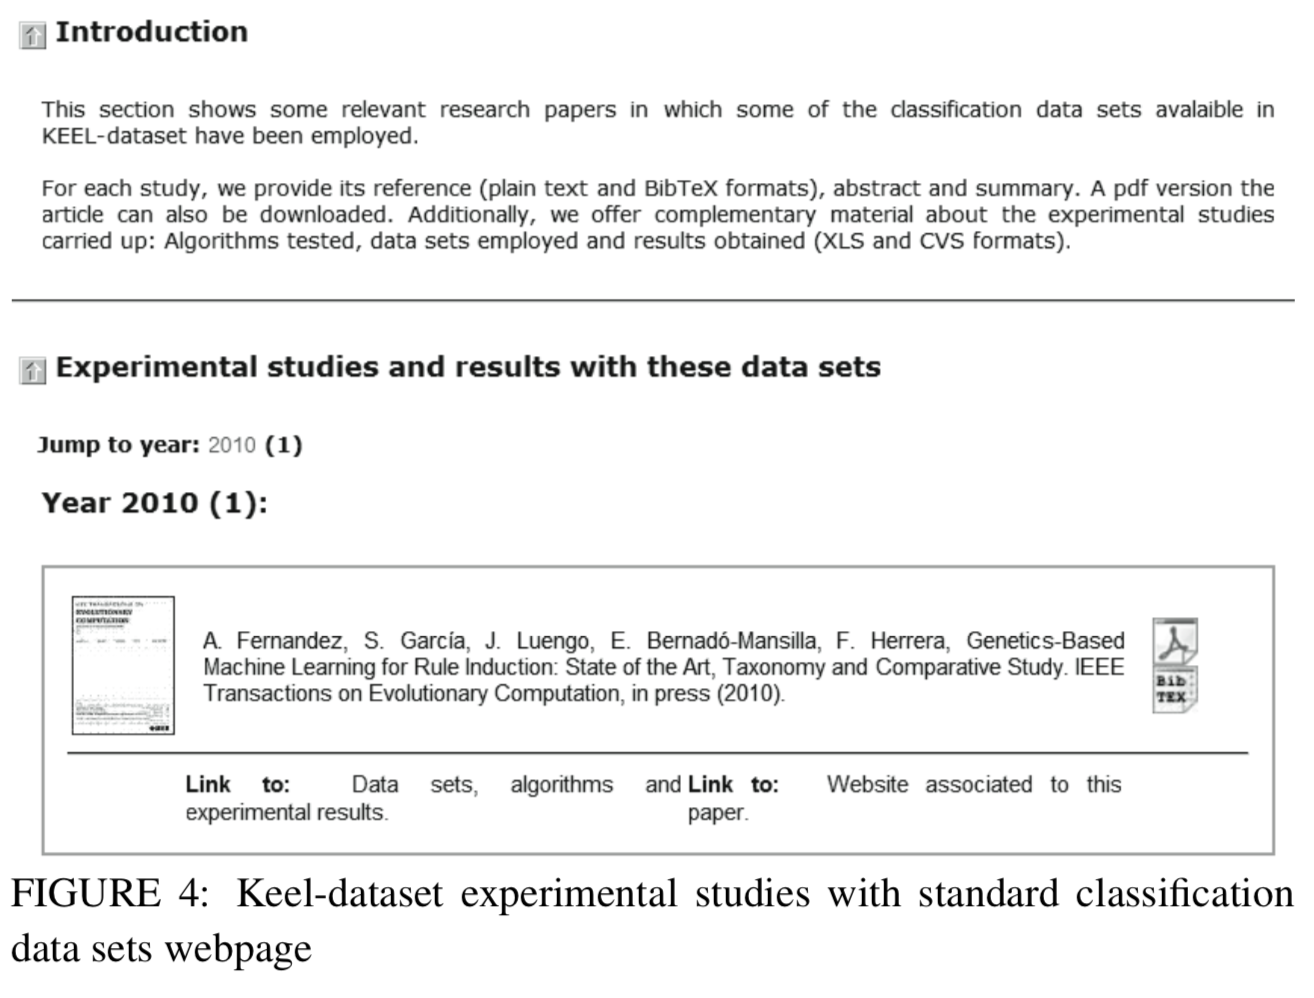
\includegraphics[height=.6\textheight]{./3.png}
\end{center}
\end{frame}

%------------------------------------------------

%------------------------------------------------

\begin{frame}
	\frametitle{\insertsection : \insertsubsection}

	\begin{block}{ i.e}
		~\\
		\centering\textbf{$R = IF~ X_{1}~ is~ [0.0,5.0[ ~and ~X_{2} ~is~ [5.0,10.0]~~ → C_{1}$}\\
		~\\
		\centering\textbf{$wWRAcc'  (R)=\dfrac{1.0+0.5}{1.0+1.0+0.0+1.0+0.5}\bullet(\dfrac{1.0+0.5}{1.0+0.5}-\dfrac{2}{5})$}\\
		~\\
		=~0.257.~~~~~~~~~~~~~~~~~~~~~~~~~~~~~
		~\\
	\end{block}
	
	
\end{frame}

%------------------------------------------------

%------------------------------------------------

\begin{frame}
	\frametitle{\insertsection : \insertsubsection}
	
	\begin{block}{ (10)}
		~\\
		\centering\textbf{$wWRAcc''  (A\longrightarrow C_{j})=\dfrac{n''(A\bullet C_{j})}{n'(C_{j})}\bullet(\dfrac{n''(A\bullet C_{j})}{n''(A)}-\dfrac{n(C_{j})}{N})$}\\
		~\\
	\end{block}
{\small 		\begin{itemize}
			\item n"(A) is the sum of the products of the weights of all covered patterns by their matching degrees with the antecedent part of the rule.
			\item n"(A · $C_{j}$ ) is the sum of the products of the weights of all correctly covered patterns by their matching degrees with the antecedent part of the rules.
			\item n′($C_{j}$ ) is the sum of the weights of patterns of class $C_{j}$.
			\item Moreover, the first term
			in the definition of wWRAcc′ has been replaced by $\dfrac{n''(A\bullet C_{j})}{n'(C_{j})}$ to reward rules that cover uneliminated patterns of class $C_{j}$ .
		\end{itemize}}
	
\end{frame}

%------------------------------------------------

%------------------------------------------------

\begin{frame}
	\frametitle{\insertsection : \insertsubsection}

	\begin{block}{i.e }
	~\\
		\centering\textbf{$wWRAcc"  (R)=\dfrac{1.0\ast1.0+0.5\ast0.5}{1.0+0.5}\bullet(\dfrac{1.0\ast1.0+0.5\ast0.5}{1.0\ast1.0+0.5\ast0.5}-\dfrac{2}{5})$}\\
		~\\
		=~0.5.~~~~~~~~~~~~~~~~~~~~~~~~~~~~~
		~\\
	\end{block}
			\begin{itemize}
				\item This measure can obtain positive or negative values in the interval \\~ [ - 1.0, 1.0]. 
				\item A rule with a wWRAcc" value near to 1 may be more useful for the classification.
			\end{itemize}
	
\end{frame}

%------------------------------------------------

\subsection{Stage 3. Rule Selection and Lateral Tuning}

%------------------------------------------------
\begin{frame}
	\frametitle{\insertsection : \insertsubsection}

\begin{center}
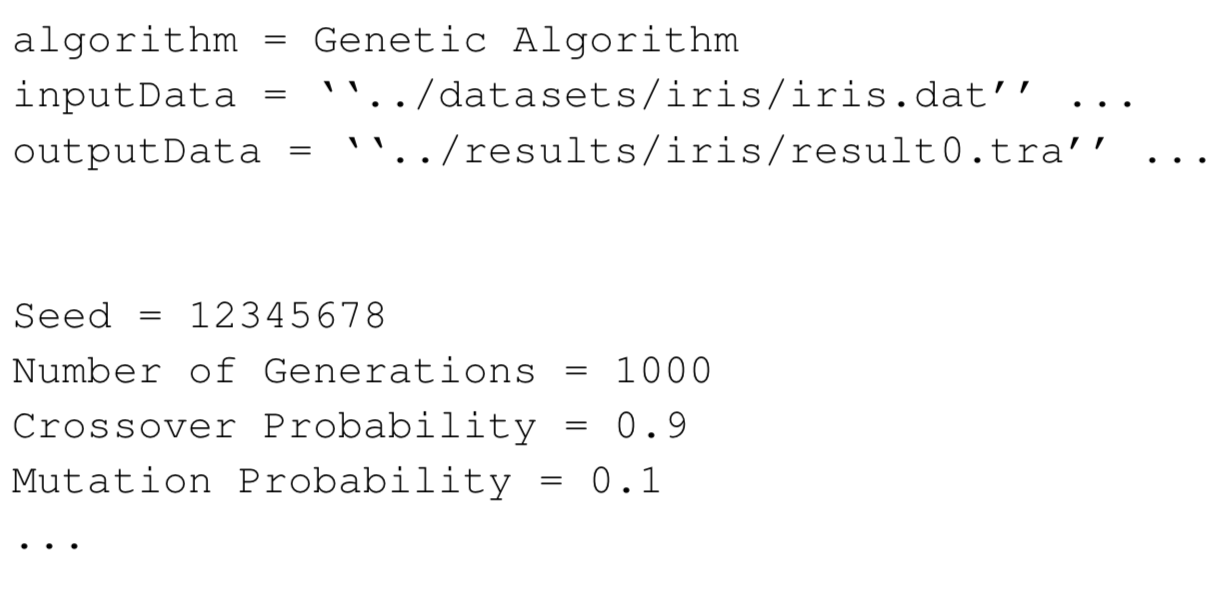
\includegraphics[height=.6\linewidth]{./4.png}
\end{center}
\end{frame}
%------------------------------------------------

%------------------------------------------------
\begin{frame}
	\frametitle{\insertsection : \insertsubsection}
	
\begin{center}
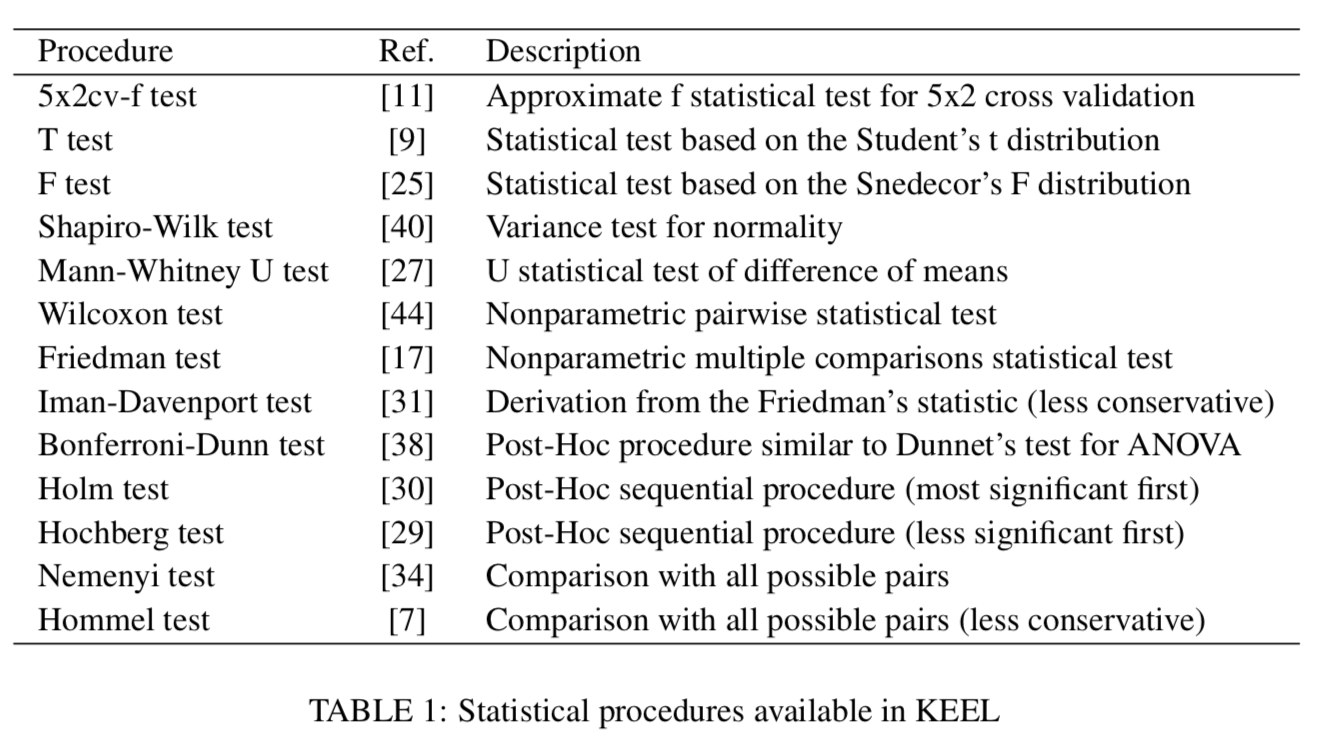
\includegraphics[height=.65\textheight]{./5.png}
\end{center}
\end{frame}
%------------------------------------------------

%------------------------------------------------

\begin{frame}
	\frametitle{\insertsection : \insertsubsection}
	
		\begin{itemize}
			\item Fig. 3.
			of the involved MF. (a) Simbolic translation of a linguistic term. (b) Lateral displacement of an MF.
		\end{itemize}
	\begin{block}{Classic Rule: }
		~\\
		\centering\textbf{$IF ~X_{1}~ is ~Low ~and~ X_{2}~ is~ Middle $}\\
			\centering\textbf{$THEN~ Class~ is~ C_{1}$}\\
		~\\

	\end{block}
		\begin{block}{Two-Tuple Representation:}
			~\\
			\centering\textbf{$IF ~X_{1}~ is~ (Low, 0.1)~ and ~X_{2}~ is~ (Middle, -0.3)$}\\
			\centering\textbf{$THEN ~Class~ is~C_{1} .$}\\
			~\\

		\end{block}

	
\end{frame}

%------------------------------------------------

%------------------------------------------------

\begin{frame}
	\frametitle{\insertsection : \insertsubsection}
	the main characteristics of the genetic approach that combines rule selection and lateral tuning are presented:
	\begin{itemize}
		\item  genetic model
		\item codification
		\item initial gene pool
		\item chromosome evaluation
		\item crossover operator
		\item restarting approach
	\end{itemize}
	\begin{block}{ }
		~\\
		\textbf{1) CHC Genetic Model}\\
		\textbf{2) Codification and Initial Gene Pool}\\
		\textbf{3) Chromosome Evaluation}\\
		\textbf{4) Crossover Operator}\\
		~\\
	\end{block}

\end{frame}

%------------------------------------------------

%------------------------------------------------
\begin{frame}
	\frametitle{\insertsection : \insertsubsection}
	
	\begin{center}
		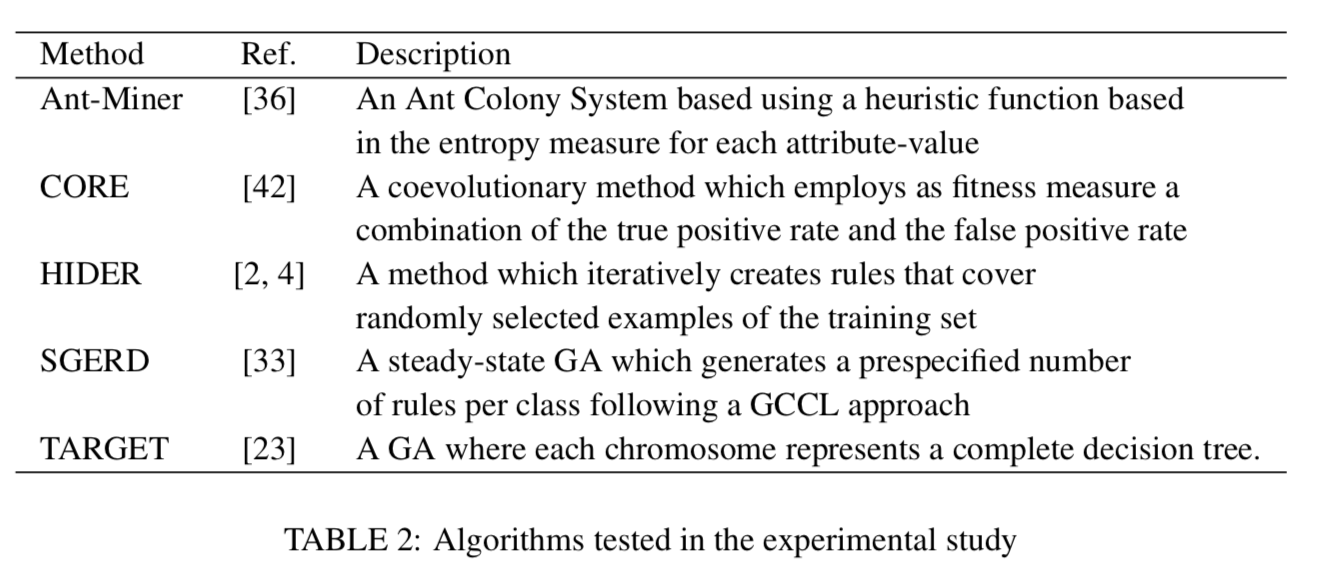
\includegraphics[height=.65\textheight]{./6.png}
	\end{center}
\end{frame}
%------------------------------------------------

\subsection{Flowchart}

%------------------------------------------------
\begin{frame}
	\frametitle{\insertsection : \insertsubsection}
	
	\begin{center}
		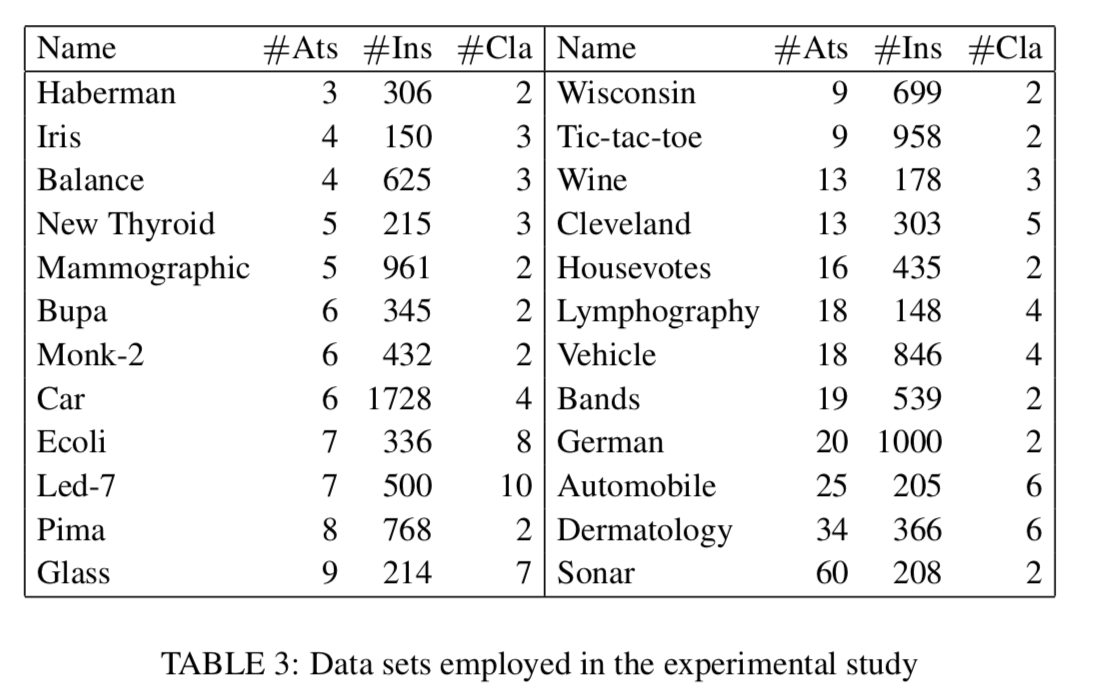
\includegraphics[height=.65\textheight]{./7.png}
	\end{center}
\end{frame}
%------------------------------------------------
%------------------------------------------------
\begin{frame}
	\frametitle{\insertsection : \insertsubsection}
	
	\begin{center}
		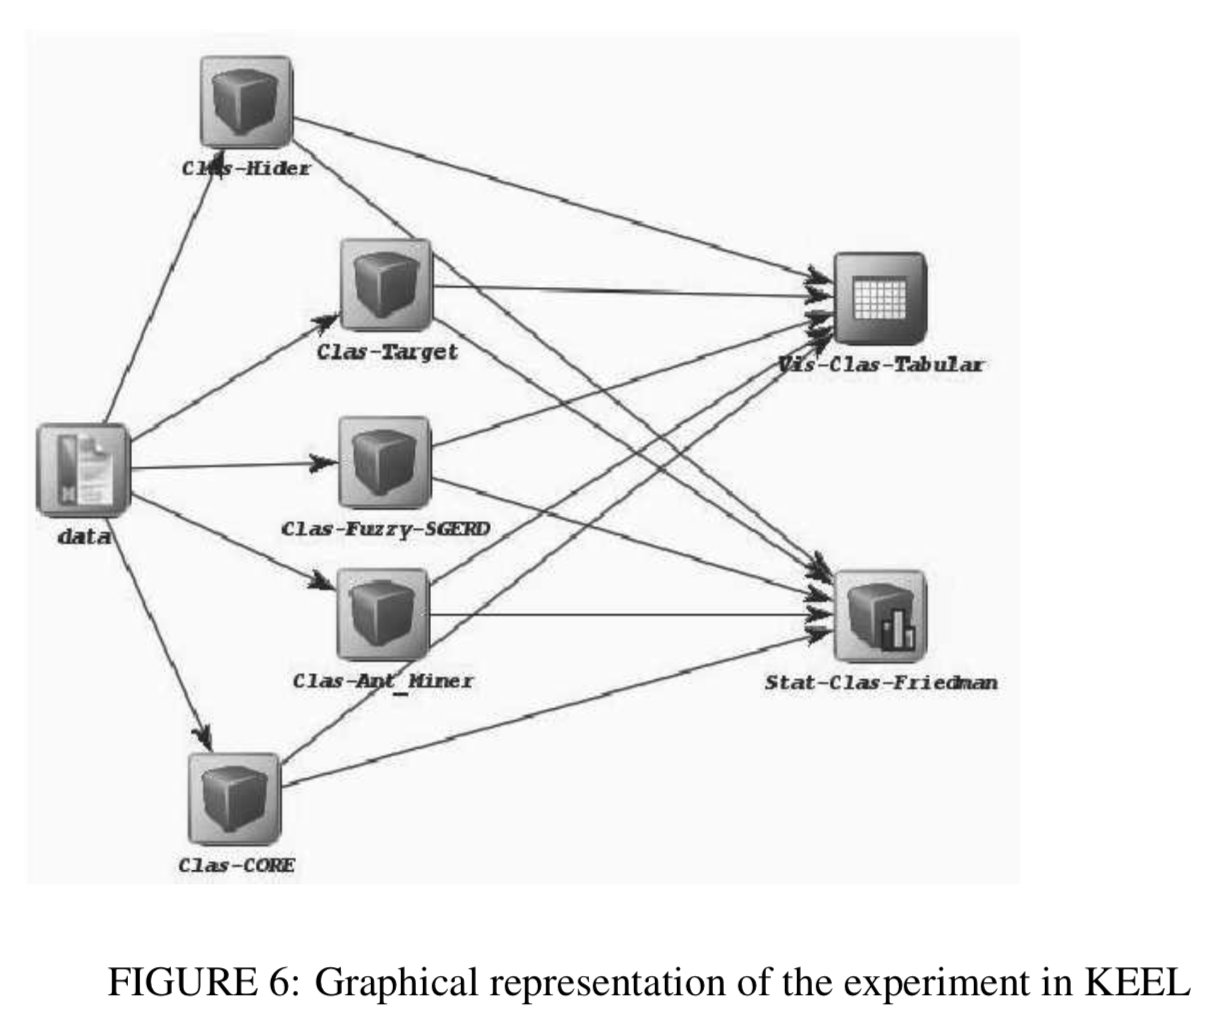
\includegraphics[height=.65\textheight]{./8.png}
	\end{center}
\end{frame}
%------------------------------------------------

\section{EXPERIMENTAL SETUP}
%------------------------------------------------

\begin{frame}
	\frametitle{\insertsection : \insertsubsection}
	Several experiments have been carried out in this paper to evaluate the usefulness of our proposal.
	\begin{itemize}
		\item we describe the real-world databases that are used in these experiments.
		\item we introduce a brief description of the methods considered for comparison.
		\item we show the configuration of the methods (determining all the parameters used).
		\item we describe the statistical analysis that is adopted in this study.
	\end{itemize}
\end{frame}

%------------------------------------------------
\subsection{A.Datasetst}

%------------------------------------------------
\begin{frame}
	\frametitle{\insertsection : \insertsubsection}
	
	\begin{center}
		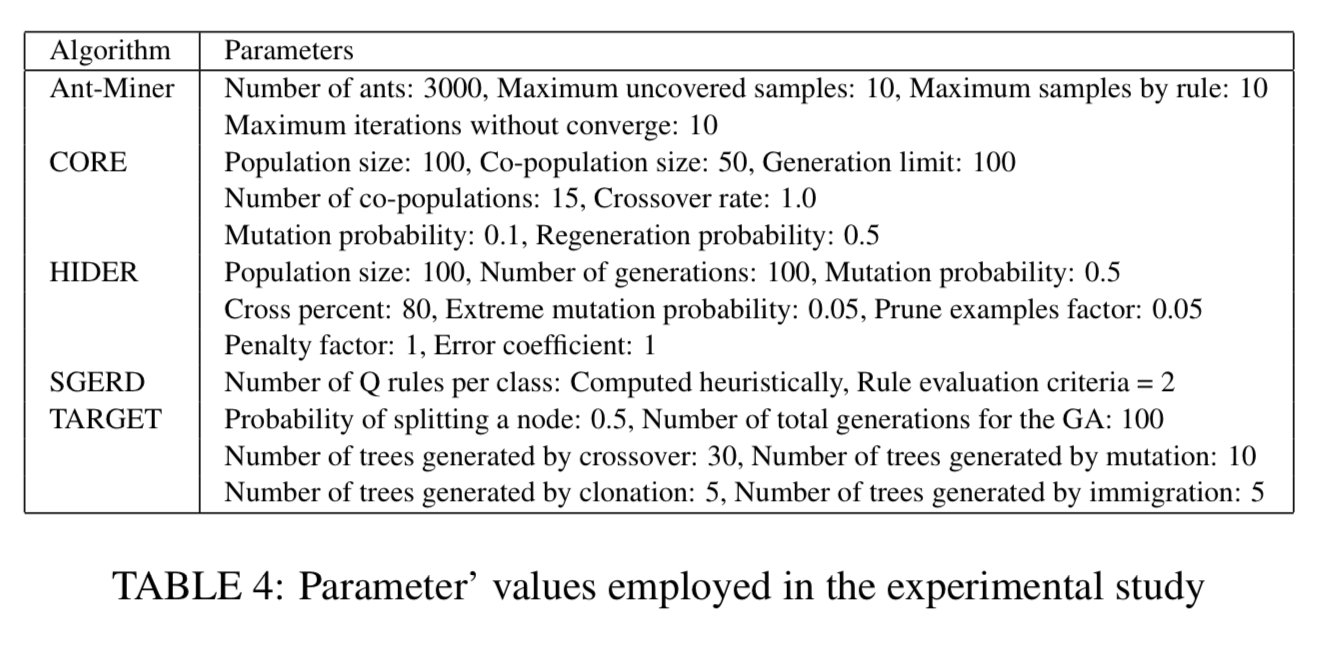
\includegraphics[height=.7\textheight]{./9.png}
	\end{center}
\end{frame}
%------------------------------------------------

\subsection{B.Methods Considered for Comparison}

%------------------------------------------------

\begin{frame}
	\frametitle{\insertsection : \insertsubsection}
	In these experiments, we compare the proposed approach with other ten methods, which are available in the Knowledge Extraction based on Evolutionary Learning (KEEL) software tool [61].
{\footnotesize 	\begin{itemize}
		\item C4.5 [39]
		\item Classification based on associations (CBA) [12]
		\item CBA2 [13]
		\item Classification based on multiple association rules (CMAR) [14]
		\item Structural learning algorithm on vague environment (2SLAVE) [64]
		\item Learning algorithm to discover fuzzy association rules for classification (LAFAR) [24]
		\item Classification based on predictive association rules (CPAR) [15]
		\item Fuzzy hybrid genetic-based machine learning algo- rithm (FH-GBML) [66]
		\item Steady-state GA for extracting fuzzy classification rules
from data (SGERD) [67]
		\item Classification with fuzzy association rules (CFAR) [27]
	\end{itemize}}
\end{frame}

%------------------------------------------------

\subsection{C.Parameters of the Methods}

%------------------------------------------------
\begin{frame}
	\frametitle{\insertsection : \insertsubsection}
	
	\begin{center}
		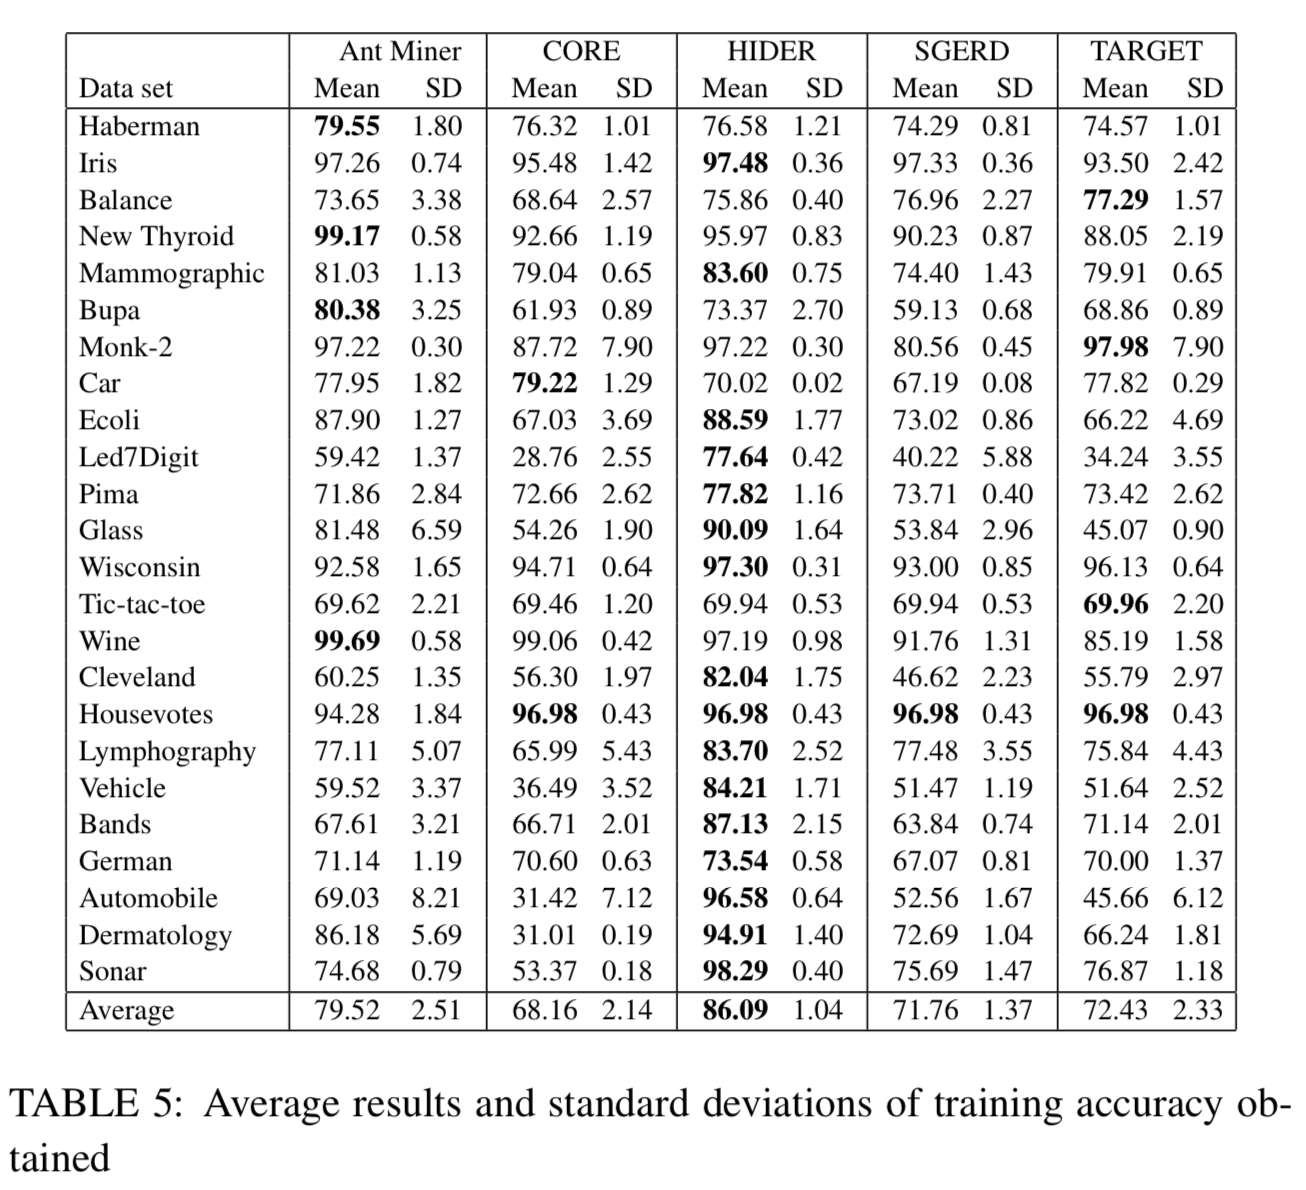
\includegraphics[height=.7\textheight]{./10.png}
	\end{center}
\end{frame}
%------------------------------------------------

\subsection{D.Statistical Analysis}

%------------------------------------------------

\begin{frame}
	\frametitle{\insertsection : \insertsubsection}
	\begin{itemize}
			\item We use α = 0.05 as the level of confidence in all cases. 
			\item A wider description of these tests, together with software for their use, can also be found at: http://sci2s.ugr.es/sicidm/
	\end{itemize}
	\begin{center}
				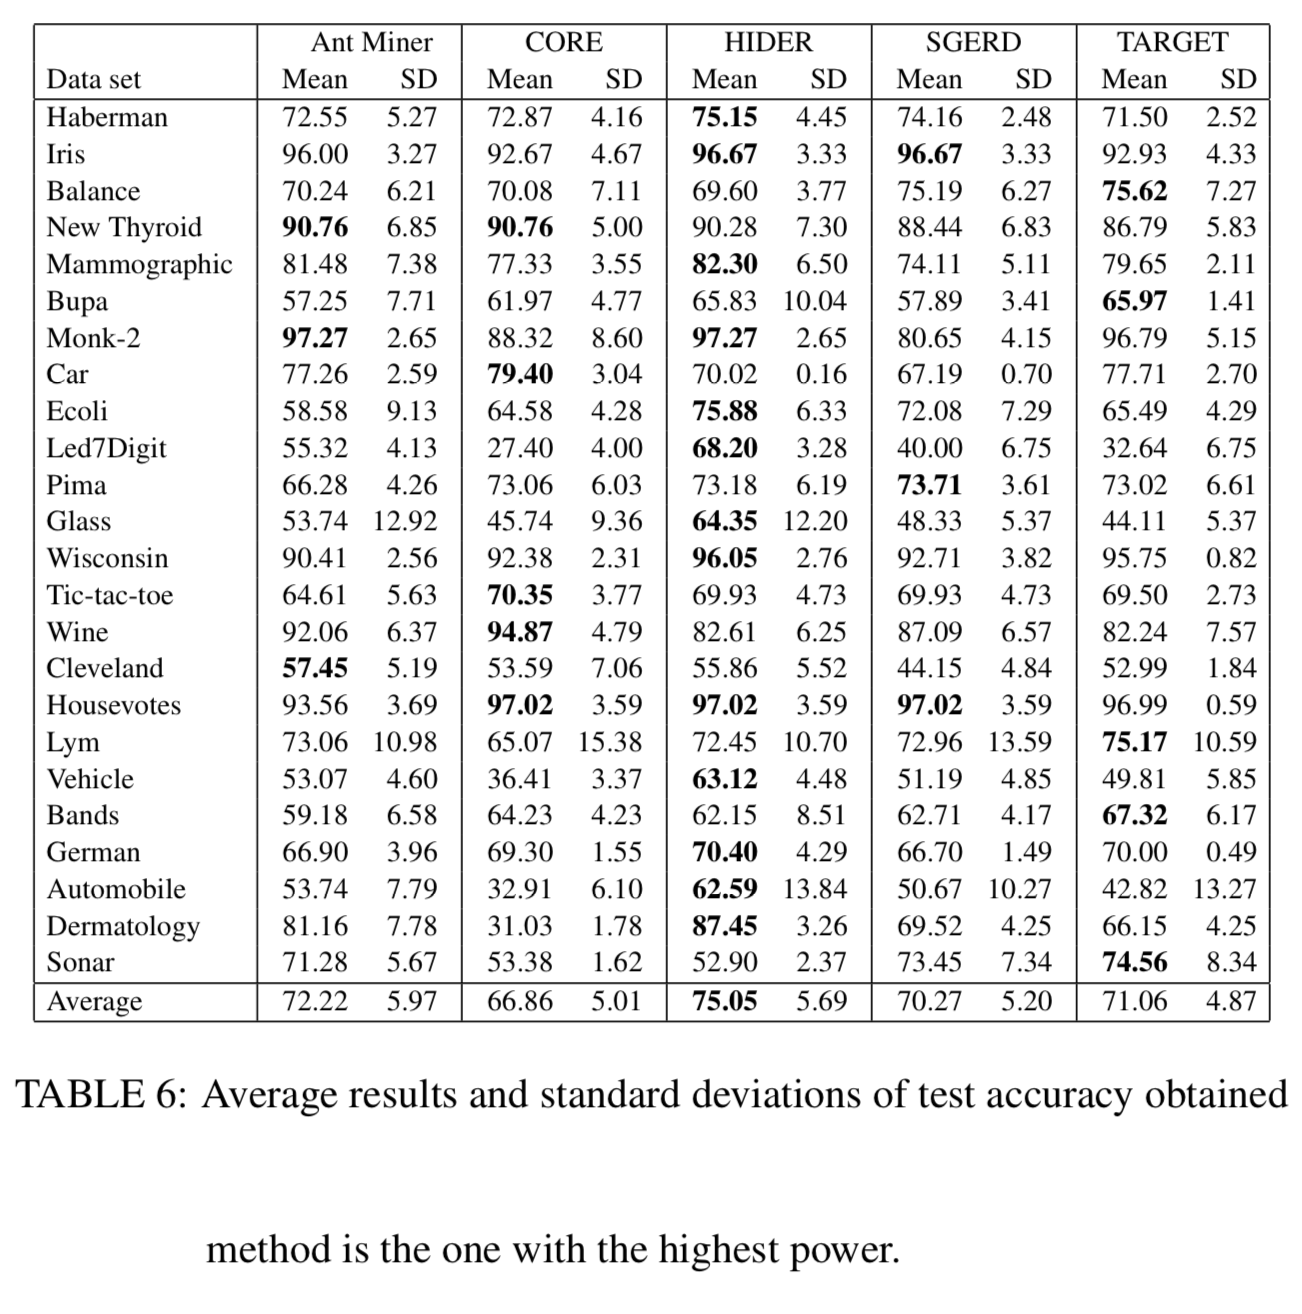
\includegraphics[height=.7\textheight]{./11.png}
	\end{center}
\end{frame}
	
%------------------------------------------------


\section{EXPERIMENTAL RESULTS}
\subsection{A.Comparison With Other Genetic Fuzzy Systems}

%------------------------------------------------

\begin{frame}
	\frametitle{\insertsection : \insertsubsection}
	\begin{center}
		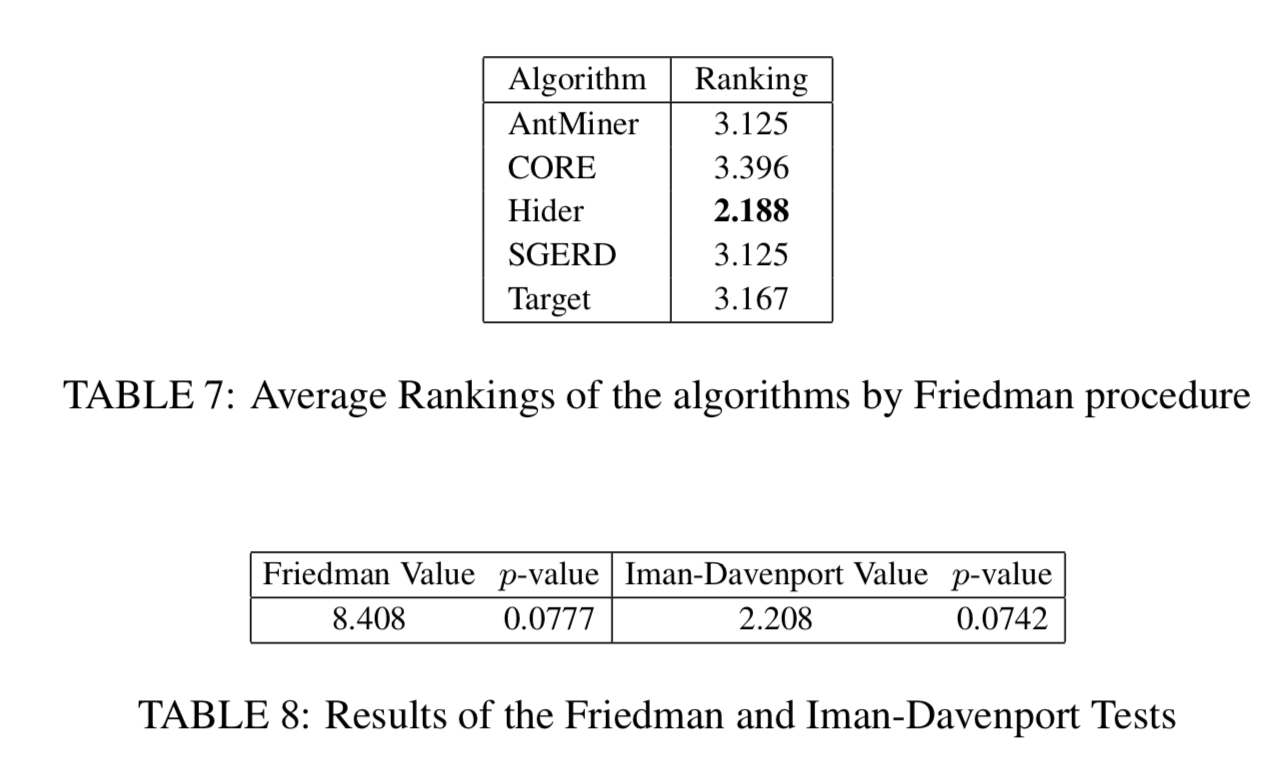
\includegraphics[height=.75\textheight]{./12.png}
	\end{center}
\end{frame}

%------------------------------------------------
%------------------------------------------------

\begin{frame}
	\frametitle{\insertsection : \insertsubsection}
\begin{center}
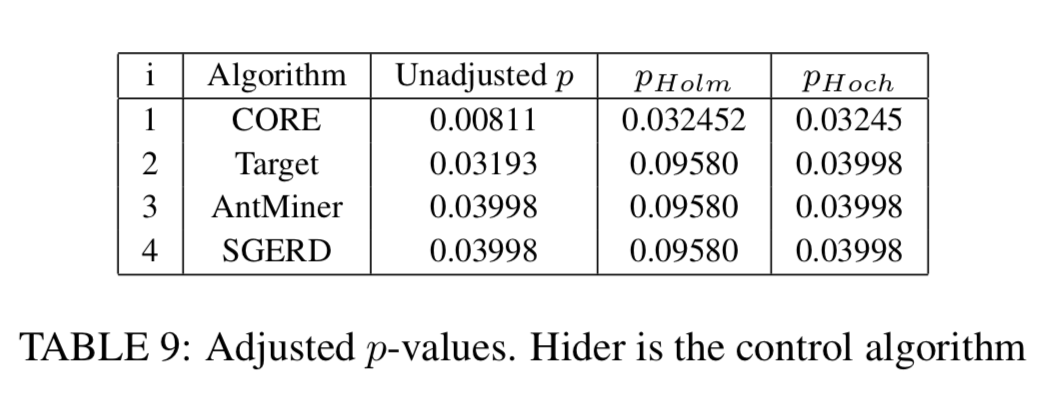
\includegraphics[width=1\linewidth]{./13.png}
\end{center}
\end{frame}

%------------------------------------------------
%------------------------------------------------

\begin{frame}
	\frametitle{\insertsection : \insertsubsection}
	\begin{center}
		\includegraphics[width=1\textheight]{./14.png}
	\end{center}
\end{frame}

%------------------------------------------------
%------------------------------------------------

\begin{frame}
	\frametitle{\insertsection : \insertsubsection}
	\begin{center}
		\includegraphics[width=1\textheight]{./15.png}
	\end{center}
\end{frame}

%------------------------------------------------

\subsection{B.Comparison With Other Fuzzy Associative Classifiers}

%------------------------------------------------

\begin{frame}
	\frametitle{\insertsection : \insertsubsection}
	\begin{center}
		\includegraphics[height=.75\textheight]{./16.png}
	\end{center}
\end{frame}

%------------------------------------------------
%------------------------------------------------

\begin{frame}
	\frametitle{\insertsection : \insertsubsection}
	\begin{itemize}
		\item The results obtained by these methods are shown in Table VIII. 
		\item Notice that we show less datasets; this is due to scalability problems in the LAFAR and CFAR algorithms, which cannot run in all datasets.
		\item On the other hand, the results presented in Table VIII show that our approach obtains an average number of rules lower than the LAFAR and CFAR algorithms.
		\item However, the CFAR algorithm obtains less rules than our approach in 11 of the 18 datasets.
	\end{itemize}
\end{frame}

%------------------------------------------------
%------------------------------------------------

\begin{frame}
	\frametitle{\insertsection : \insertsubsection}
	\begin{center}
		\includegraphics[width=1\textheight]{./17.png}
	\end{center}
	In order to compare the two algorithms, we use a Wilcoxon test, which is shown in Table IX.
\end{frame}

%------------------------------------------------

\subsection{C.Comparison With Classical Approaches}

%------------------------------------------------

\begin{frame}
	\frametitle{\insertsection : \insertsubsection}
	\begin{center}
		\includegraphics[height=.75\textheight]{./18.png}
	\end{center}
\end{frame}

%------------------------------------------------
%------------------------------------------------

\begin{frame}
	\frametitle{\insertsection : \insertsubsection}
	\begin{center}
		\includegraphics[width=1\textheight]{./19.png}
	\end{center}
\end{frame}

%------------------------------------------------
%------------------------------------------------

\begin{frame}
	\frametitle{\insertsection : \insertsubsection}
	\begin{center}
		\includegraphics[width=1\textheight]{./20.png}
	\end{center}
\end{frame}

%------------------------------------------------
%------------------------------------------------

\begin{frame}
	\frametitle{\insertsection : \insertsubsection}
	\begin{center}
		\includegraphics[width=1\textheight]{./21.png}
	\end{center}
\end{frame}

%------------------------------------------------

\subsection{D.Analysis of the Influence of $Depth_{max}$ and the Number of Evaluations}
%------------------------------------------------

\begin{frame}
	\frametitle{\insertsection : \insertsubsection}
	ANALYSIS OF THE PERFORMANCE DEPENDING ON $Depth_{max}$
	\begin{center}
		%\includegraphics[width=1\textheight]{./22.png}
		\includegraphics[height=.75\textheight]{./22-1.png}
	\end{center}
\end{frame}

%------------------------------------------------
%------------------------------------------------

\begin{frame}
	\frametitle{\insertsection : \insertsubsection}
	\begin{center}
		\includegraphics[width=1\textheight]{./23.png}
	\end{center}
\end{frame}

%------------------------------------------------

\subsection{E.Analysis of Scalability}

%------------------------------------------------

\begin{frame}
	\frametitle{\insertsection : \insertsubsection}
	\begin{center}
		\includegraphics[width=1\textheight]{./24.png}
	\end{center}
\end{frame}

%------------------------------------------------
%------------------------------------------------

\begin{frame}
	\frametitle{\insertsection : \insertsubsection}

	\begin{block}{By the analysis of the results presented in Table XV, we can draw the following conclusions. }
		~\\
	\begin{itemize}
		\item The SGERD algorithm presents a very low average runtime in all datasets.
		\item The 2SLAVE,FH-GBML,LAFAR ,and CFAR algorithms expend a large amount of time .\\ (Notice that the CFAR and LAFAR cannot run in 7 and 18 of the 26 datasets, respectively.)
		\item our proposal obtains the best ranking in Fried- man’s test .
		\item Notice that the CBA and CBA2 algorithms present similar runtimes to the CMAR and CPAR algorithms.
		\item The FARC-HD approach presents a good computational cost in all datasets.
	\end{itemize}
		~\\
	\end{block}
	
\end{frame}

%------------------------------------------------

\section{CONCLUDING REMARKS}

%------------------------------------------------

\begin{frame}
	\frametitle{\insertsection : \insertsubsection}
	

		\begin{itemize}
			\item In this paper, we have proposed a new fuzzy associative clas- sification method for high-dimensional datasets, named FARC-HD.
			\item Our aim was to obtain accurate and compact fuzzy asso- ciative classifiers with a low computational cost.
			\item Finally, the limit in the depth of the trees, along with candidate rule prescreening using the fuzzy measure wWRACC", allows us to reduce the search space considerably.
		\end{itemize}

	
\end{frame}

%------------------------------------------------

%%------------------------------------------------
%
%\begin{frame}
%\frametitle{4.1 Fuzzy Measures}
%A set function g defined on \Large $\mathscr{B}$ \normalsize that has the following properties is called a {\color{red}fuzzy measure}:\\
%\begin{block}{Definition 4-1}
%
%~\\
%1. g(0)=0,g(X)=1.\\
%2. If A,B $\in$\Large $\mathscr{B}$\normalsize~ and A$ \subseteq $B,then g(A) $\leq$ g(B).\\
%3. If $A_{n}~\in$ \Large $\mathscr{B}$\normalsize,$A_{1} \subseteq A_{2} \subseteq$...,then $ \lim_{n \rightarrow  \infty } $($A_{n}$)=g($ \lim_{n \rightarrow  \infty } A_{n}$).\\
%~\\
%\end{block}
%Sugeno's measure differs from the classical measure essentially by relaxing the additivity property [Murofushi and Sugeno 1989, p. 201].\\
%A different approach,however, is used by Klement and Schwyhla [1982].\\
%The interested reader is referred to their article.
%\end{frame}
%
%%------------------------------------------------
%%------------------------------------------------
%
%\begin{frame}
%\frametitle{4.1 Fuzzy Measures}
%Banon [1981] shows that very many measures with finite universe, such as probability measures, belief functions, plausibility measures, and so on, are fuzzy measures in the sense of Sugeno. \\
%For this book, one measure-possibility-is of particular interest [see Dubois and Prade 1988a, p.7].\\
%In the framework of fuzzy set theory, Zadeh introduced {\color{red}the notion of a possibility distribution and the concept of a possibility measure}, which is a special type of the fuzzy measure proposed by Sugeno. \\
%A possibility measure is defined as follows [Zadeh 1978; Higashi and Klir 1982]:
%
%\end{frame}
%
%%------------------------------------------------
%%------------------------------------------------
%
%\begin{frame}
%\frametitle{4.1 Fuzzy Measures}
%Let P(X) be the power set of a set X.\\
%A possibility measure is a function $ \Pi $: P(X) $ \mapsto $ [0, 1] with the properties\\
%\begin{block}{Definition 4-2}
%l. $ \Pi $(0)=0,$ \Pi $(X)=1\\
%2. A $ \subseteq $ B $ \Rightarrow  \Pi   $(A) $\leq \Pi $(B)\\
%3. $\Pi$ ($U_{i \in I}A_{i}$ ) = $sup_{i\in I} \Pi$ ($A_{i}$) with an index set I.
%~\\
%\end{block}
%It can be uniquely determined by a possibility distribution function f: X $ \rightarrow $ [0, 1] by$\Pi$(A)=$sup_{x \in A}f$ f(x),A $\subset$ X.\\
%It follows directly that f is defined by f(x) =$\Pi$(\{x\})$\forall_x \in X$ ~[Klir and Folger 1988, p. 122].\\
%A possibility is not always a fuzzy measure [Puri and Ralescu 1982].\\
%It is, however, a fuzzy measure if X is finite and if the possibility distribution is normal-that is, a mapping into [0, 1].
%\end{frame}
%
%%------------------------------------------------
%%------------------------------------------------
%
%\begin{frame}
%\frametitle{4.1 Fuzzy Measures}
%
%\begin{block}{Example 4-1}
%Let X = {0, 1, . . . , 10} .\\
%$\Pi$(\{x\}) : = Possibility that x is close to 8.\\
%~\\
%\begin{table}[h]
%\begin{tabular}{|l|l|l|l|l|l|l|l|l|l|l|l|}
%\hline
%x  & 0  & 1  & 2 & 3 & 4 & 5 & 6 & 7 & 8 & 9 & 10 \\ \hline
%$\Pi$(\{x\}) & .0 & .0 & .0  & .0  & .0 & .1 & .5 & .8 & 1 & .8 & .5 \\ \hline
%\end{tabular}
%\end{table}
%~\\
%$\Pi$(A): = Possibility that A contains an integer close to 8.\\
%A $\subset$~X$~ \Longrightarrow~$ $\Pi$(A) = $sup_{x \in A}$ $\Pi$(\{x\}) \\
%For A = {2, 5, 9} we compute:\\
%$\Pi$(A) = $sup_{x \in A}$ $\Pi$(\{x\}) \\
%= sup\{$\Pi$(\{2\}), $\Pi$(\{5\}), $\Pi$(\{9\})\} \\
%= sup\{0, .1, .8\}\\
%=.8\\
%~\\
%~\\
%\end{block}
%
%\end{frame}
%
%%------------------------------------------------
%
%%\subsection{4.2 Measures of Fuzziness} 
%
%%------------------------------------------------
%
%\begin{frame}
%\frametitle{4.2 Measures of Fuzziness}
%
%\begin{itemize}
%\item Measures of fuzziness, in contrast to fuzzy measures, try to indicate {\color{red}the degree of fuzziness of a fuzzy set.} 
%\item A number of approaches to this end have become known. 
%\item Some authors, strongly influenced by the \textbf{Shannon entropy} as a measure of information, and following de Luca and Termini [1972], consider a measure of fuzziness as {\color{red}a mapping \textbf{d} from the power set P(X) to [0, +\(\infty \)] that satisfies a number of conditions}.
%
%\item Others [Kaufmann 1975] suggested an index of fuzziness as a \textbf{normalized distance}, and others [Yager 1979; Higashi and Klir 1982] base their concept of a measure of fuzziness on \textbf{the degree of distinction between the fuzzy set and its complement}.
%
%\end{itemize}
%
%\end{frame}
%
%%------------------------------------------------
%
%%------------------------------------------------
%
%\begin{frame}
%\frametitle{4.2 Measures of Fuzziness}
%We shall, as an illustration, discuss two of those measures.\\
%Suppose for both cases that \textbf{the support of A is finite}.\\
%~\\
%The first is as follows : Let $\mu_{\tilde{A}}(x)$ be the membership function of the fuzzy set $\tilde{A}$ for $x \in X$, X finite. It seems plausible that the measure of fuzziness d($\tilde{A}$) should then have the following properties [de Luca and Termini 1972]:\\
%\begin{block}{}
%\begin{itemize}
%\item1. d($\tilde{A}$) = 0 if $\tilde{A}$ is a crisp set in X.
%\item2. d($\tilde{A}$) assumes a unique maximum if $\mu_{\tilde{A}}(x)$ = $ \frac{1}{2} \forall x \in X$.
%\item3. d($\tilde{A}) \geq  d(\tilde{A'}$) if $\tilde{A'}$ is "crisper" than $\tilde{A}$, i.e., if $\mu_{\tilde{A'}}(x) \leq$ $\mu_{\tilde{A}}(x)$ for $\mu_{\tilde{A}}(x) \leq \frac{1}{2}$ and  $\mu_{\tilde{A'}}(x) \geq$ $\mu_{\tilde{A}}(x)$ for $\mu_{\tilde{A}}(x) \geq \frac{1}{2}$. 
%\item4. d(¢$\tilde{A}$) = d($\tilde{A}$) where ¢$\tilde{A}$ is the complement of $\tilde{A}$.
%\end{itemize}
%\end{block}
%\end{frame}
%
%%------------------------------------------------
%%------------------------------------------------
%
%\begin{frame}
%\frametitle{4.2 Measures of Fuzziness}
%De Luca and Termini suggested as a measure of fuzziness the {\color{red}"entropy"} of a fuzzy set [de Luca and Termini 1972, p. 305], which they defined as follows :\\
%\begin{block}{Definition 4-3a}
%The entropy as a measure of a fuzzy set $\tilde{A}$ = \{(x, $\mu_{\tilde{A}}(x))$\} is defined as\\
%~\\
%\centering\textbf{d($\tilde{A}$) = H($\tilde{A}$) + H(¢$\tilde{A}$), x $\in$ X}\\
%\centering\textbf{H($\tilde{A}$) = - K$\sum_{i=1}^n \mu_{\tilde{A}}(x_{i})ln(\mu_{\tilde{A}}(x_{i}))$}\\
%~\\
%\end{block}
%where \textbf{n} is the number of elements in the support of $\tilde{A}$ and K is a positive constant.
%\end{frame}
%
%%------------------------------------------------
%%------------------------------------------------
%
%\begin{frame}
%\frametitle{4.2 Measures of Fuzziness}
%Using \textbf{Shannon's function S(x)=-xlnx-(1-x)ln(1-x)}, de Luca and Termini simplify the expression in definition 4-3a to arrive at the following definition.\\
%\begin{block}{Definition 4-3b}
%The entropy d as a measure of fuzziness of a fuzzy set $\tilde{A}$ = \{x, $\mu_{\tilde{A}}(x)$\} is defined as\\
%~\\
%\centering\textbf{d($\tilde{A}$) = K$\sum_{i=1}^n S(\mu_{\tilde{A}}(x_{i}))$}\\
%~\\
%\end{block}
%\end{frame}
%
%%------------------------------------------------
%%------------------------------------------------
%
%\begin{frame}
%\frametitle{4.2 Measures of Fuzziness}
%\begin{block}{Example 4-2}
%Let $\tilde{A}$= "integers close to 10" (see example 2-1d)\\
%~~~~~~~~~~~~$\tilde{A}$ = \{(7, .1), (8, .5), (9, .8), (10, 1),(11, .8), (12, .5), (13,.1)\}\\
%Let K = 1, so\\
%~~~~~~~~~~~~d($\tilde{A}$) = .325+.693+.501+0+.501+.693+.611+.325=3.038\\
%~\\
%Furthermore, let $\tilde{B}$ ="integers quite close to 10"\\
%~~~~~~~~~~~~$\tilde{B}$ = \{(6,.1),(7,.3),(8,.4),(9,.7),(10,1),(11,.8),(12,.5),(13,.3),(14,.l)\}\\
%~~~~~~~~~~~~d($\tilde{B}$) = .325 +.611+.673+.611+0+.501+.693+.611+.325=4.35
%\end{block}
%
%\begin{block}{Shannon's function \textbf{S(x)=-xlnx-(1-x)ln(1-x)}}
%\centering\textbf{$\mu_{\tilde{A}}(x)$=0.1,\\
%-$\mu_{\tilde{A}}(x)$ln($\mu_{\tilde{A}}(x)$)-(1-$\mu_{\tilde{A}}(x)$)ln(1-$\mu_{\tilde{A}}(x)$)\\
%=-0.1ln(0.1)-(1-0.1)ln(1-0.1)\\
%$ \approx $0.325}\\
%\end{block}
%\end{frame}
%
%%------------------------------------------------
%%------------------------------------------------
%
%\begin{frame}
%\frametitle{4.2 Measures of Fuzziness}
%The second measure is as follows: Knopfmacher [1975], Loo [1977], Gottwald [1979b], and others based their contributions on the Luca and Termini's suggestion in some respects.\\
%~~\\
%If $\tilde{A}$ is a fuzzy set in X and ¢$\tilde{A}$ is its complement, then in contrast to crisp sets, \textbf{it is not necessarily true} that\\
%\begin{block}{}
%~\\
%~\\
%\centering\textbf{$\tilde{A}~  \cup$  ¢$\tilde{A}$ = X}\\
%\centering\textbf{$\tilde{A}~  \cap$~~¢$\tilde{A}$ = \(\phi\) }\\
%~\\
%\end{block}
%This means that \textbf{fuzzy sets do not always satisfy the law of the excluded middle}, which is one of their major distinctions from traditional crisp sets. \\
%~~\\
%Some authors [Yager 1979; Higashi and Klir 1982] consider the relationship between $\tilde{A}$ and ¢$\tilde{A}$ to be the essence of fuzziness.
%\end{frame}
%
%%------------------------------------------------
%%------------------------------------------------
%
%\begin{frame}
%\frametitle{4.2 Measures of Fuzziness}
%Yager [1979] notes that the requirement of distinction between $\tilde{A}$ and ¢$\tilde{A}$ \textbf{is not satisfied by fuzzy sets}.
%\\
%He therefore suggests that any measure of fuzziness \textbf{should be a measure of the lack of distnction between $\tilde{A}$ and ¢$\tilde{A}$ or $\mu_{\tilde{A}}(x)~ and~ \mu_{~~~¢\tilde{A}}(x)$}.\\
%As a possible metric to measure the distance between a fuzzy set and its complement, Yager suggests:\\
%\begin{block}{Definition 4-4}
%~\\
%~\\
%\centering\textbf{\(D_{p}( \tilde{A},~~¢\tilde{A}) = [~ \sum_{i=1}^n   | \mu_{\tilde{A}}( x_{i}) - \mu_{~~~¢\tilde{A}}( x_{i} ) |^{p} ~]^ \frac{1}{p}  ~~~~p=1,2,3...\)}\\
%~\\
%\raggedright Let S ~=~supp($\tilde{A}$): $D_{p}$(S, ¢S) =~$\|S\|^\frac{1}{p}$\\
%~\\
%\end{block}
%
%\end{frame}
%
%%------------------------------------------------
%%------------------------------------------------
%
%\begin{frame}
%\frametitle{4.2 Measures of Fuzziness}
%
%\begin{block}{Definition 4-5[Yager 1979](1/2)}
%~\\
%~\\
%A measure of the fuzziness of $\tilde{A}$ can be defined as\\
%~\\
%\centering\textbf{$f_{p}(\tilde{A})$ = 1 - $\frac{D_{p}(\tilde{A},~~~¢\tilde{A})}{\|supp(\tilde{A})\|}$}\\
%~\\
%\raggedright So $f_{p}$($\tilde{A}$) $\in$ [0, 1]. This measure also satisfies properties 1 to 4 required by de Luca and Termini (see above).\\
%~\\
%~\\
%\end{block}
%
%\end{frame}
%
%%------------------------------------------------
%%------------------------------------------------
%
%\begin{frame}
%\frametitle{4.2 Measures of Fuzziness}
%
%\begin{block}{Definition 4-5[Yager 1979](2/2)}
%~\\
%~\\
%For p = 1, $D_{p}$($\tilde{A}$, ¢$\tilde{A}$) yields \textbf{the Hamming metric}\\
%~\\
%\centering\textbf{$D_{1}(\tilde{A},~~¢\tilde{A})$ = $\sum_{i=1}^n |\mu_{\tilde{A}}( x_{i})- \mu_{~~~¢\tilde{A}}( x_{i} )| $}\\
%~\\
%\raggedright Because $\mu_{\textbf{¢}\tilde{A}}( x) = 1 - \mu_{\tilde{A}}( x)$, this becomes\\
%~\\
%\centering\textbf{$D_{1}(\tilde{A},~~¢\tilde{A})$ = $\sum_{i=1}^n |2\mu_{\tilde{A}}( x_{i})- 1| $}\\
%~\\
%\raggedright For p = 2, we arrive at \textbf{the Euclidean metric}\\
%~\\
%\centering\textbf{$D_{2}(\tilde{A},~~¢\tilde{A})$ = $(\sum_{i=1}^n (\mu_{\tilde{A}}( x_{i})- \mu_{~~~¢\tilde{A}}( x_{i} ))^2 )^ \frac{1}{2} $}\\
%~\\
%\raggedright and for $\mu_{\textbf{¢}\tilde{A}}( x) = 1 - \mu_{\tilde{A}}( x)$, we have\\
%~\\
%\centering\textbf{$D_{2}(\tilde{A},~~¢\tilde{A})$ = $(\sum_{i=1}^n (2\mu_{\tilde{A}}( x_{i})- 1 ))^2 )^ \frac{1}{2} $}\\
%~\\
%\end{block}
%
%\end{frame}
%
%%------------------------------------------------
%%------------------------------------------------
%
%\begin{frame}
%\frametitle{4.2 Measures of Fuzziness}
%
%\begin{block}{Example 4-3(1/2)}
%~\\
%Let $\tilde{A}$ = "integers close to 10" and\\
%$\tilde{B}$ = "integers quite close to 10" be defined as in {\color{red}example 4-2.}\\
%Applying the above derived formula, we compute for p = 1:\\
%~\\
%\centering\textbf{$D_{1}(\tilde{A},~~¢\tilde{A})$ =.8+0+.6+1+.6+0+.8}\\
%\textbf{=3.8}\\
%\centering\textbf{$\|supp(\tilde{A})\| = 7$}\\
%\raggedright so $f_{1}(\tilde{A}) = 1 - \frac{3.8}{7}$ = {\color{red}0.457.}\\
%~\\
%Analogously,\\
%\centering $D_{2}(\tilde{B},\textbf{¢}\tilde{B})$ = 4.6\\
%\centering\textbf{$\|supp(\tilde{B})\| = 9$}\\
%\raggedright so $f_{1}(\tilde{B}) = 1 - \frac{4.6}{9}$ = {\color{red}0.489.}\\
%~\\
%~\\
%\end{block}
%
%\end{frame}
%
%%------------------------------------------------
%%------------------------------------------------
%
%\begin{frame}
%\frametitle{4.2 Measures of Fuzziness}
%
%\begin{block}{Example 4-3(2/2)}
%~\\
%~\\
%Similarly, for p = 2, we obtain\\
%\centering $D_{2}(\tilde{A},\textbf{¢}\tilde{A})$ = 1.73\\
%\centering\textbf{$\|supp(\tilde{A})\| = 2.65$}\\
%\raggedright so $f_{2}(\tilde{A}) = 1 - \frac{1.73}{2.65}$ = {\color{red}0.347} ,and\\
%~\\
%\centering $D_{2}(\tilde{B},\textbf{¢}\tilde{B})$ = 1.78\\
%\centering\textbf{$\|supp(\tilde{B})\| = 1$}\\
%\raggedright so $f_{2}(\tilde{B}) = 1 - \frac{1.78}{3}$ = {\color{red}0.407.}\\
%~\\
%~\\
%\end{block}
%
%\end{frame}
%
%%------------------------------------------------
%%------------------------------------------------
%
%\begin{frame}
%\frametitle{4.2 Measures of Fuzziness}
%
%\begin{itemize}
%\item The reader should realize that {\color{red}the complement of a fuzzy set is not uniquely defined} [see Bellman and Giertz 1973; Dubois and Prade 1982a; Lowen 1978]. 
%\item It is therefore not surprising that for other definitions of the complement and for other measures of distance, other measures of fuzziness will result, even though they all focus on the distinction between a fuzzy set and its complement [see, for example, Klir 1987, p. 141]. 
%\item Those variations, as well as {\color{red}extension of measures of fuzziness to nonfinite supports, will not be considered here}; neither will the approaches that define fuzzy measures of fuzzy sets [Yager 1979].
%
%\end{itemize}
%
%\end{frame}
%
%%------------------------------------------------
%------------------------------------------------
\begin{frame}
\Huge{\centerline{Thank you for your attention}}
\end{frame}

%----------------------------------------------------------------------------------------

\clearpage\end{CJK*}
\end{document}